\subsection{Text-Based Retrieval-Augmented Generation}
\subsubsection{Retrieval-Augmented Generation}

Retrieval-Augmented Generation (RAG) combines a generator with an external information store. Lewis et al.~\cite{lewis2020rag} formulated a neural retrieval-and-generation model in 2020 using a dense index of Wikipedia; the general paradigm therefore predates the document-specific examples discussed here. For document QA, the distinctive problem is to preserve and recover evidence across sections, pages, and documents under a bounded input budget. Retrieval can reduce the context passed to a generator, but it introduces a selection bottleneck: a generator cannot reliably use evidence that the retriever has omitted. We distinguish retrieval representation (passages, hierarchy, or graph) from runtime control (fixed or iterative retrieval), because either representation can be used with either control strategy. These are composable design choices, not successive levels of reasoning ability. Representative retrieve-then-generate and multi-hop approaches include the following. Triple-Fact Retriever \cite{wu2022triple} improved the accuracy and interpretability of cross-document evidence paths in multi-hop DocQA by extracting structured triple facts and aggregating evidence hop by hop. Multi-Document Question Answering with Lightweight Embeddings-based Document Reranker \cite{aitymbetov2024multi} employed a two-stage retrieval process combining BM25 coarse-ranking with lightweight embedding-based re-ranking, improving evidence quality in multi-document QA while maintaining efficiency. Zero-Shot Complex Question-Answering on Long Scientific Documents \cite{wang2025zero} integrated RAG with question decomposition, multi-hop reasoning, and long-answer generation, achieving complex QA on long documents without task-specific fine-tuning. Meanwhile, DR-RAG \cite{hei2024dr} mitigated evidence omission in multi-hop QA caused by static similarity retrieval by introducing dynamic document relevance modeling and a two-stage filtering mechanism.

\subsubsection{Structure-Aware Evidence Access}

Building on traditional RAG improvements centered on retrieval quality and multi-hop support, subsequent research began to focus further on utilizing the reasoning capabilities of LLMs and internal or cross-document structural information to construct more structure-aware and reasoning-guided retrieval-augmentation frameworks. Among these, DocReLM: Mastering Document Retrieval with Language Model \cite{wei2024docrelm} fine-tuned retrievers and re-rankers by introducing LLMs to generate domain-specific training data and utilized LLM-generated citation networks to expand candidate document sets, thereby significantly enhancing semantic understanding and cross-literature association discovery in academic literature retrieval. Advanced Chain-of-Thought Reasoning for Parameter Extraction from Documents Using Large Language Models \cite{chen2025advanced} introduced an improved chain-of-thought reasoning mechanism into document-level information extraction tasks, achieving reasoning-driven refined retrieval and parameter localization through modules such as Targeted Document Retrieval, Iterative Retrieval Optimization, and Preference Optimization. Semi-Structured Chain-of-Thought: Integrating Multiple Sources of Knowledge for Improved Language Model Reasoning \cite{su2024semi} further explored the unification of parametric knowledge, structured knowledge graphs, and unstructured text retrieval into a semi-structured reasoning chain, allowing multi-source knowledge to be progressively filled and integrated during the reasoning process. In long-document scenarios, Beyond Chunking: Discourse-Aware Hierarchical Retrieval for Long Document Question Answering \cite{chen2025chunkingdiscourseawarehierarchicalretrieval} utilized Rhetorical Structure Theory (RST) for discourse-level modeling of documents and performed hierarchical retrieval on this structure, effectively alleviating the issue of semantic incoherence caused by flat chunking. For multi-document scenarios, Knowledge Graph Prompting for Multi-Document Question Answering \cite{wang2024knowledge} enhanced global consistency and multi-document reasoning capabilities by constructing cross-document knowledge graphs and guiding the LLM through graph-traversal evidence collection. Meanwhile, PdfTriage: Question Answering over Long, Structured Documents \cite{saad2024pdftriage} focused on structured long-document QA, explicitly modeling structural meta-information such as pages, sections, and tables to enable RAG to accurately respond to queries containing structural references. These methods show how document structure can guide evidence access. Their common trade-off is that useful hierarchy or relations must first be recovered or constructed; a structural index should therefore be evaluated for both retrieval coverage and the errors introduced during its construction.

\subsubsection{Graph and Hierarchical Evidence Indexes}

Graph and hierarchical indexes expose relations that flat passages may conceal, but an index structure should not be conflated with an agentic policy. Some systems prepare graphs and summaries offline and answer through a predefined query workflow; others adapt the next retrieval action to intermediate observations. Both can support multi-hop questions, and either can fail through incomplete or incorrectly linked evidence. From Local to Global: A Graph RAG Approach to Query-Focused Summarization \cite{edge2024graphrag} (GraphRAG) proposed a graph-enhanced retrieval framework based on knowledge graphs and community detection, addressing global, cross-document summarization queries by constructing entity-relationship graphs and generating community summaries. Subsequently, LightRAG: Simple and Fast Retrieval-Augmented Generation \cite{guo2024lightrag} proposed a dual-level retrieval design intended to reduce the overhead of graph-enhanced retrieval while retaining access to entity and relational information. Furthermore, HyperGraphRAG: Retrieval-Augmented Generation via Hypergraph-Structured Knowledge Representation \cite{he2024hypergraphrag} used hyperedges to represent relations involving multiple entities directly, rather than organizing all evidence as pairwise links. This changes the representation of a relation, but does not itself establish that the extracted relation is correct. Leveraging Spreading Activation for Improved Document Retrieval in Knowledge-Graph-Based RAG Systems \cite{pavlovic2025leveraging} enabled activation values to propagate dynamically along evidence chains for prioritized retrieval of relevant fragments by automatically constructing knowledge graphs and executing spreading activation, serving as a plug-and-play module that enhanced multi-hop evidence continuity in chain-based reasoning. GARLIC: LLM-Guided Dynamic Progress Control with Hierarchical Weighted Graph for Long Document QA \cite{wang2024garlic} constructed a hierarchical weighted directed acyclic graph based on LLM attention for dynamic retrieval, allowing retrieval paths and information volume to be adaptively controlled by the LLM, overcoming the limitations of traditional vector similarity and fixed tree summarization. For multi-document environments, HiQA: A Hierarchical Contextual Augmentation RAG for Multi-Documents QA \cite{chen2024hiqa} transformed documents into hierarchical structures with cascading metadata and fused vector, BM25, and keyword matching through multi-path retrieval to improve retrieval discriminability in structurally similar document sets. For complex hierarchical documents, BookRAG: A Hierarchical Structure-aware Index-based Approach for Retrieval-Augmented Generation on Complex Documents \cite{wang2025bookrag} built BookIndex, fusing logical hierarchy trees and entity-relationship graphs, and introduced an agentic retrieval strategy inspired by information foraging theory to dynamically select retrieval workflows, thereby balancing recall, efficiency, and multi-hop path integrity. In multi-hop reasoning, Enhancing Document-Level Question Answering via Multi-Hop Retrieval-Augmented Generation with LLaMA 3 \cite{huang2025enhancing} integrated dense retrieval, context fusion, and multi-hop mechanisms, strengthening retrieval-generation synergy through the joint optimization of retrieval likelihood and generation loss. Finally, Chain of Retrieval: Multi-Aspect Iterative Search Expansion and Post-Order Search Aggregation for Full Paper Retrieval \cite{park2025chain} drove iterative expansion retrieval via multi-aspect decomposition and reorganized hierarchical evidence through post-order aggregation, reflecting a paradigm shift in which the retrieval process itself served as the reasoning chain. The resulting design space combines evidence organization with control policy. A graph can support global aggregation without interactive search, whereas iterative retrieval can operate over ordinary passages. Consequently, the effect of graph construction should be separated from the effect of extra retrieval or generation calls when comparing systems.

\begin{figure*}[t]
\centering
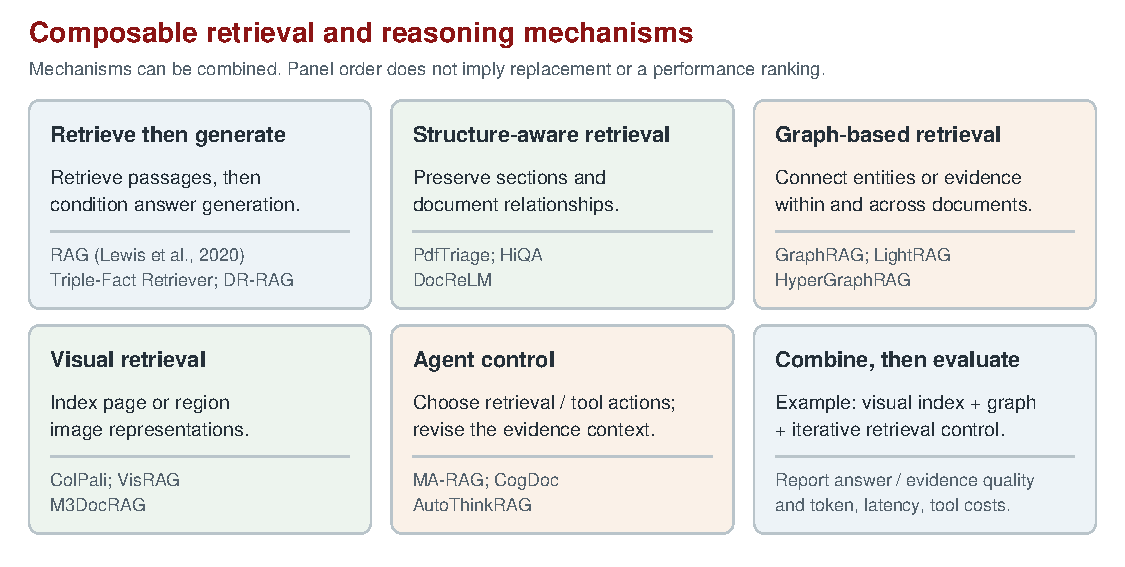
\includegraphics[
    width=0.95\textwidth,
    height=0.38\textheight,
    keepaspectratio,
    trim=0cm 0cm 0cm 0cm,
    clip
]{figs_by_qixingyu/fig06.pdf}
\caption{Composable retrieval-augmented mechanisms for document QA, arranged as a grid rather than a performance timeline: retrieve-then-generate, structure-aware access, graph-based organization, visual retrieval, and agent control. The RAG formulation dates to Lewis et al. (2020); mechanisms may be combined, and each combination requires explicit accuracy and resource evaluation.}
\label{fig:rag_evolution}
\end{figure*}

\subsubsection{Text QA Foundations and Their Scope}

\paragraph{Early Attention Mechanisms}
Before contemporary generative RAG, text QA research studied how to select and combine evidence from supplied passages. These methods provide historical context for textual evidence reasoning; they do not address all of the visual and geometric constraints of document images. Dynamic Coattention Networks \cite{dynamiccoattention2017} proposed a co-attention strategy to capture bidirectional interaction information by simultaneously attending to the question and the document. Addressing the excessive search range in long documents, Coarse-to-fine question answering \cite{coarsetofine2017} pioneered a "coarse-to-fine" two-stage framework: first retrieving relevant sentences, then extracting precise answers. To further enhance text representation capabilities, EA Reader \cite{eareader2019} utilized multi-space context fusion to improve performance in cloze-style QA.

\paragraph{Reasoning Based on Graph Structures and Global Information}
As document length and complexity continued to increase, Graph Neural Networks (GNNs) offered one approach to connecting discrete pieces of textual evidence. Question Answering by Reasoning Across Documents with GCNs \cite{gcnmultihop2019} was among the earliest works to utilize entity-based Graph Convolutional Networks for handling multi-hop tasks. Subsequently, Identifying Supporting Facts with Document Graph Networks \cite{dgn2019} further shifted the research focus from answer prediction to the explicit identification of supporting facts. This shift was achieved by modeling multi-document contexts as sentence-level document graphs and introducing question-conditioned GNN reasoning mechanisms on the graph structure. Meanwhile, the Heterogeneous Graph approach \cite{heterograph2019} handled cross-document reasoning by modeling different types of nodes (e.g., entities, documents). In recent research, Path-based GCN \cite{pathgcn2020} emphasized reasoning along specific relational paths, while Capturing global structural information in long document question answering with compressive graph selector network \cite{cgsn2022} achieved more efficient long-document QA through integrated global structural encoding.

To improve the capability and interpretability of multi-hop QA, researchers began exploring explicit reasoning chains and explainable frameworks. First, Exploiting Explicit Paths \cite{explicitpaths2019} proposed that the key lay in selecting a correct evidence path, with the model scoring and choosing within a path space. Multi-hop Question Answering via Reasoning Chains \cite{reasoningchains2020} proposed the use of "reasoning chains" as intermediate explicit variables, where the model predicted one or more reasoning chains before generating an answer. Explore, Propose, and Assemble \cite{epa2019} proposed a three-stage explainable reasoning framework to bridge information fragments. Further progress in explainability included Select, Answer and Explain \cite{sae2020}, which simultaneously generated answers and evidence rationales, elevating "explanation" from an auxiliary task to an output as important as the answer itself. Hop, Union, Generate \cite{hug2023} proposed guiding the model to form an explainable reasoning process without explicit evidence supervision. Additionally, Ask to Understand \cite{asktounderstand2023} proposed revealing complex multi-hop logic clearly by generating a series of intermediate questions.

\paragraph{Task Generalization and the LLM Era}
Work on translation~\cite{multihoptransformer2021}, relation extraction~\cite{syntaxmultihop2024}, and script-event prediction~\cite{docscript2024} provides adjacent methodological background for multi-hop modeling. We do not treat those tasks as direct document QA benchmarks: their inputs, outputs, and supervision differ. Their relevance is limited to transferable mechanisms for combining contextual information, which require separate validation on document questions.

Within document QA, MemSum-DQA~\cite{memsumdqa2023} uses extractive summarization to shorten the material supplied to a QA model. Effect of Document Packing~\cite{documentpacking2025} examines how organizing context affects multi-hop reasoning. These methods highlight that evidence access is shaped by selection and presentation even when no external retrieval stage is exposed. Comparisons should therefore state whether a method receives a whole document, retrieved passages, a summary, or oracle evidence.

\subsubsection{Choosing Context Access and Retrieval Control}

The choice between full-context processing and retrieval depends on evidence density, corpus size, update frequency, model capacity, and resource limits. LaRA~\cite{lara2025} explicitly evaluates this choice and finds no universally preferable route. Supplying a complete document avoids a separate retrieval recall failure when the input fits, but does not ensure that a model will use every relevant passage. Retrieval is attractive when a question needs a small portion of a large or changing collection; its answer quality remains conditional on recovering all necessary evidence. A structure-aware index can preserve section membership and cross-references, while also inheriting errors in parsing or graph construction. These are different access assumptions, so reported scores should be compared only after matching the available evidence and input budget.

Iterative or agent-controlled retrieval is most directly motivated when the next information need cannot be specified before examining earlier evidence. It can, for example, follow an entity or a cross-reference discovered during the first lookup. Additional rounds also create opportunities for query drift, repeated retrieval, and propagation of an early mistaken interpretation. Our design implication is to expose a stopping rule, a maximum number of actions, evidence already inspected, and the conditions for abstention, rather than treating a longer trace as evidence of deeper reasoning. A fixed retrieval pass or direct full-context model is a necessary control when evaluating whether additional actions contribute useful evidence.

The resulting comparison should decompose failures into evidence coverage, evidence selection, and answer use. An oracle-evidence setting isolates the reader from the retriever; an end-to-end setting measures their joint behavior. Removing a cited passage, substituting a distractor, or checking the answer against a retrieved source can further probe whether the answer is supported by the evidence. Such checks assess different properties from a plausible explanation or a successful retrieval call. This framework links text-based RAG to table and visual document QA through a shared requirement: retain source identity while selecting, transforming, and using evidence.
